%%%%%%%%%%%%%%%%%%%%%%%%%%%%%%%%%%%%%%%%%%%%%%%%%%%%%%%%%%%%%%%%%%%%
%% I, the copyright holder of this work, release this work into the
%% public domain. This applies worldwide. In some countries this may
%% not be legally possible; if so: I grant anyone the right to use
%% this work for any purpose, without any conditions, unless such
%% conditions are required by law.
%%%%%%%%%%%%%%%%%%%%%%%%%%%%%%%%%%%%%%%%%%%%%%%%%%%%%%%%%%%%%%%%%%%%

\documentclass[
  digital, %% This option enables the default options for the
           %% digital version of a document. Replace with `printed`
           %% to enable the default options for the printed version
           %% of a document.
  table,   %% Causes the coloring of tables. Replace with `notable`
           %% to restore plain tables.
  lof,     %% Prints the List of Figures. Replace with `nolof` to
           %% hide the List of Figures.
  lot,     %% Prints the List of Tables. Replace with `nolot` to
           %% hide the List of Tables.
  %% More options are listed in the user guide at
  %% <http://mirrors.ctan.org/macros/latex/contrib/fithesis/guide/mu/sci.pdf>.
]{fithesis3}
%% The following section sets up the locales used in the thesis.
\usepackage[resetfonts]{cmap} %% We need to load the T2A font encoding
\usepackage[T1,T2A]{fontenc}  %% to use the Cyrillic fonts with Russian texts.
\usepackage[
  main=english,  %% By using `czech` or `english` as the main locale
                %% instead of `slovak`, you can typeset the thesis
                %% in either Czech or English, respectively.
  english, german, russian, czech, slovak %% The additional keys allow
]{babel}        %% foreign texts to be typeset as follows:
%%
%%   \begin{otherlanguage}{german}  ... \end{otherlanguage}
%%   \begin{otherlanguage}{russian} ... \end{otherlanguage}
%%   \begin{otherlanguage}{czech}   ... \end{otherlanguage}
%%   \begin{otherlanguage}{slovak}  ... \end{otherlanguage}
%%
%% For non-Latin scripts, it may be necessary to load additional
%% fonts:
\usepackage{paratype}
\def\textrussian#1{{\usefont{T2A}{PTSerif-TLF}{m}{rm}#1}}
%%
%% The following section sets up the metadata of the thesis.
\thesissetup{
    date            = \the\year/\the\month/\the\day,
    university      = mu,
    faculty         = sci,
    department      = Ústav chemie,
    departmentEn    = Department of Chemistry,
    extra = {
      departmentCs  = Department of Chemistry,
    },
    programme       = Fyzikální chemie,
    programmeEn     = Physical Chemistry,
    extra = {
      programmeCs   = Chemistry,
    },
    field           = Fyzikální chemie,
    fieldEn         = Physical Chemistry,
    extra = {
      fieldCs       = Physical Chemistry,
    },
    type            = mgr,
    author          = Petra Hrozková,
    gender          = f,
    advisor         = doc. Markéta Munzarová Dr. rer. nat. ,
    title           = Studium elektronové struktury fosfosilikátů a jejich silikátových          prekurzorů metodou DFT,
    TeXtitle        = A DFT study of the Electronic Structure of Silicate Precursors for Phosphosilicates
.
,
    titleEn         = A DFT study of the Electronic Structure of Silicate Precursors for Phosphosilicates
,
    TeXtitleEn      = A DFT study of the Electronic Structure of Silicate Precursors for Phosphosilicates
,
    extra = {
      titleCs       =A DFT study of the Electronic Structure of Silicate Precursors for Phosphosilicates
,
      TeXtitleCs    = A DFT study of the Electronic Structure of Silicate Precursors for Phosphosilicates
,
    },
    keywords        = {kľúčové slovo 1, kľúčové slovo 2, ...},
    TeXkeywords     = {kľúčové slovo 1, kľúčové slovo 2, \ldots},
    keywordsEn      = {keyword1, keyword2, ...},
    TeXkeywordsEn   = {keyword1, keyword2, \ldots},
    extra = {
      keywordsCs    = {klíčové slovo 1, klíčové slovo 2, ...},
      TeXkeywordsCs = {klíčové slovo 1, klíčové slovo 2, \ldots},
    },
    abstract      = {This is the abstract of my thesis, which can

                     span multiple paragraphs.},
    abstractEn    = {This is the English abstract of my thesis, which can

                     span multiple paragraphs.},
    extra = {
      abstractCs   = {This is the Czech abstract of my thesis, which can

                      span multiple paragraphs.},
    },
    thanks        = {These are the acknowledgements for my thesis, which can

                     span multiple paragraphs.},
    bib           = example.bib,
    %% Uncomment the following line (by removing the % symbol at
    %% the beginning) and replace `assignment.pdf` with the
    %% filename of your scanned thesis assignment.
    % assignment    = assignment.pdf,
}
\usepackage{makeidx}      %% The `makeidx` package contains
\makeindex                %% helper commands for index typesetting.
%% These additional packages are used within the document:
\usepackage{paralist} %% Compact list environments
\usepackage{amsmath}  %% Mathematics
\usepackage{amsthm}
\usepackage{amsfonts}
\usepackage{url}      %% Hyperlinks
\usepackage{mhchem}
\usepackage{listings} %% Source code highlighting
\lstset{
  basicstyle      = \ttfamily,%
  identifierstyle = \color{black},%
  keywordstyle    = \color{blue},%
  keywordstyle    = {[2]\color{cyan}},%
  keywordstyle    = {[3]\color{olive}},%
  stringstyle     = \color{teal},%
  commentstyle    = \itshape\color{magenta}}
\usepackage{floatrow} %% Putting captions above tables
\floatsetup[table]{capposition=top}
\begin{document}




\chapter{Introduction}

\section{Experiment  X}
The goal of the thesis was to verify experimental results provided by Mgr. Aleš Stýskalík, PhD. His work was focused on silicophosphates and hypervalent silicon. Concept of hypervalent moleculs is a little bit confusing. It is possible to find a one signification for two different phenomenon. First, hypervalent molecule is a molecule with one or more elements apparently bearing more than eight electrons in their valence shells. Otherwise .... doplním podle literatury
\subsection{Silicophosphates}
Silicophosphates are important advanced-technology materials consisting of Si-O-P group most often. Silicon and phosphorus are close together in periodic table of elements hence they have similar size. For this reason, silicon and phosphorus are easily exchangeable in compounds. Both elements occur in minerals and other oxidic materials, generally surrounded by four oxygen atoms in nature. Moreover, they have extraordinary physical properties like Brønsted acidity or high proton conductivity. In future they could be applied as catalysts, electrolytes, optical glasses, and biocompatible materials. Approximative form of silicophosphates is shown in the figure \ref{si_polymer_cely}. \cite{Styskalik2015thesis} Groups of Si-O-P create poors with very variable sizes. However, it is hard to describe the exact structure of silicophosphates because silicophosphates are amorphous structure.

\subsubsection{Hypervalent silicon}
 Silicon creates binary phases, halides, hydrides or metal organic and organometallic silicon compounds. Silicon in silicophosphates is 4-, 5- and 6- coordinated and displays hypercoordinacy. Chemistry calls higher-coordinated compouds either hypercoordinated or hypervalent compounds. On the other hand, detailed explanation of higher-coordintaed compounds remains limited.
\begin{figure}[h!]
\caption{Silicophosphat's net \cite{Styskalik2015thesis}. }
  \center
  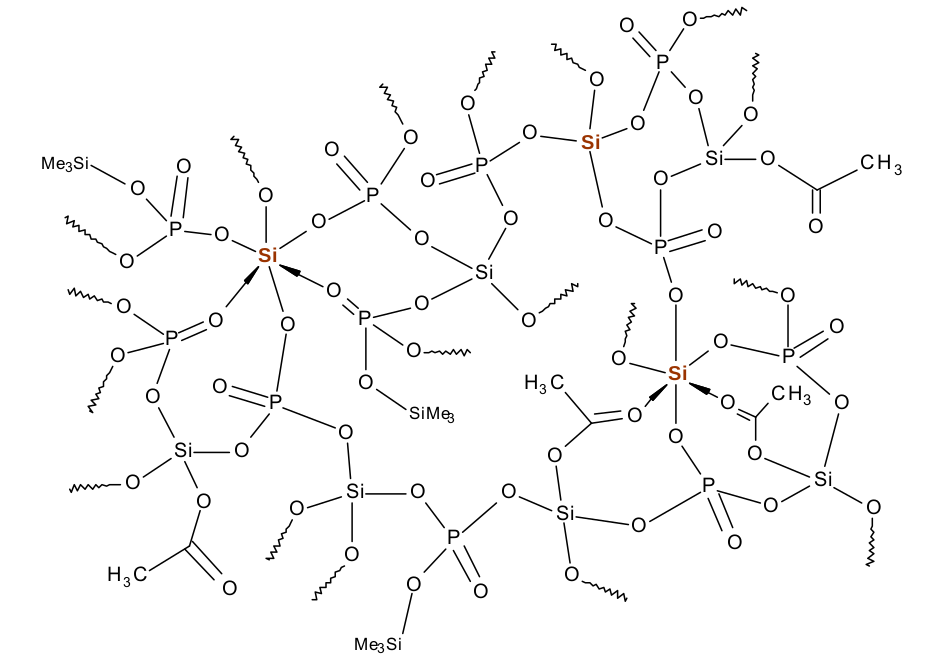
\includegraphics[width=12cm]{si_polymer_cely.png}
  \label{si_polymer_cely}
  \end{figure}
Silicon is similar to carbon, both create fourfold coordinated in most cases. Silicon observes in the third periods thus silicon has sufficient amount of orbitals in order to create five or six bonds. \ce{(SiF6)^{2-}} and \ce{(Si(NH2)2F3)^{2-}} is long known silicon structure with six bonds. First structure were already known in the nineteenth century. In the twentieth century study of silicon's compound expanded, nevertheless advanced structures were developed mostly in the last decade.
Detail analysis of acquired structure provided information and unsighted into structure and bonding in hypercoordinated silicons structures. \cite{Wagler2014}\\


\subsubsection{Physical and chemical properties}
Silicophosphates have unusual physical and chemical properties and they could be used in an industry applications. There is a strong influence of electro-negativity donors in bonds between silicon and donor's elements.  Donors such as C, N, O, F and Cl support increasing coordination of Si. The strongest electronegative element is fluor, hence first structure with hexacoordinated silicon contains six fluors. After that there was developed hexacoodinated structure with oxygen or nitrogen. In contrast, carbon is above silicon and it is capable of very different bonding characteristics. \\
Creating of hexacoordinated structure determines lewis acidity. Good lewis acid has a vacant orbital, thus structure has enough space to create another bonds. Bond between silicon and oxygens belong to a good lewis acids. In contrast, bond between silicon and carbon is little acidic thus creation hexacoodinated structure is disabled. Pentavalent silicon is better Lewis acid than fourcoordinated structure and supports hypervalency.\cite{Wagler2014}\\

\begin{figure}[h!]
\caption{\cite{hypervalentsiliconmacmillangroup2005}}
  \center
  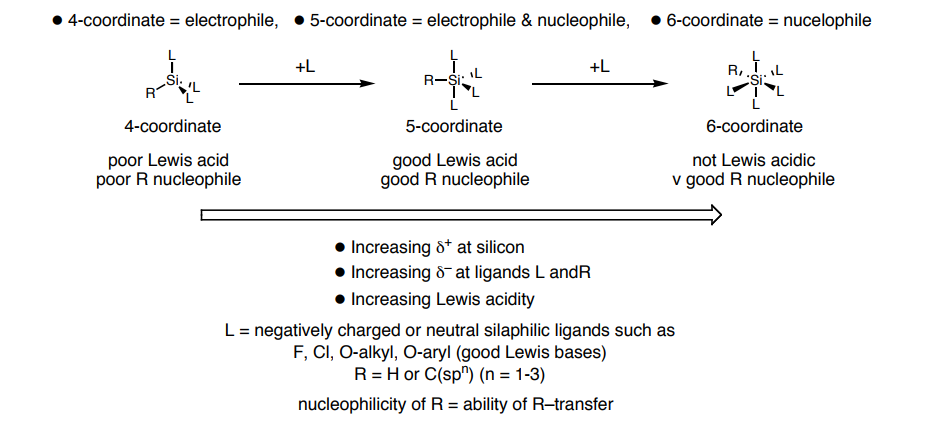
\includegraphics[width=12cm]{schema_silicophosphates.png}
  \label{schema_silicon_coordinate}
  \end{figure}


 Explanation of penta- and hexavalency was frequently discussed. First explanation of hypervalent coordination was using sp3d2 hybridization. Disadvantage of this claim is high energy of the sp3d2 hybridization. Energy of 3d orbitals is relatively high thus it is accepted that role of 3d orbital is not significant. Permission of pentavalency is determined by 3c-4e bonds, show in figure .... . Hypervalent compounds are more lewis acids because of d+ effect at the central silicon. The reason is transformation of the electron density to the ligands atoms because of non-bonding MO. This electron density distribution stabilizes structure. For this reason electronegative elements occurs in hypervalents compounds. Explanation of this phenomenon gives Ben's rule: "Electronegative elements prefer bonds with more p-character".\cite{hypervalentsiliconmacmillangroup2005} \\

 Another interpretation of hypercoordination is subsubsection namebased on the higher ionicity of the silicon bonds than in the corresponding tetrahedral species. Moreover, behavior and properties of Si-E compounds strongly depend on atom E and steric and electronis constraints. Behavior of silicon bonds can be divided into ionic, sigma bonds and dative interactions. \cite{Wagler2014}\\
For this reason we decided to compare Lewis acidity in order to determine stability of parts of silicon. Moreover we wanted to find the parameter, which determines the size of pores. I was interested in molecular orbitals, which could give us a lot of information about molecules, bonds, structure, acidity e.g. Analysis were made by density functional theory, which ranks among quantum chemistry methods. In addition, similar analysis was based on natural bond orbitals, which gets better practical view on chemical bond. Natural bond orbitals help with a transformation from a number to a chemical sense.


\section{Methods of quantum chemistry}
Chemical properties are obviously determine by electrons. Behavior of electrons is desribed by Schrödiger equation. This is a second-order differential equation and exact solution exists only for system with two particles. Therefor, it is nessesary to use an aproximation in chemical applications. The basis are Born-Oppenheimer aproximation and Slaters determinant. Born-Oppenheimer approximation assumes, that movement of nuclei and electrons can be separated. Wavefunctions is broken into two parts, electronic and nuclear \ref{B_O_approximace}. The solution reduces to 3N spatial coordinates. Furtheremore, nuclei are fixed in a certain configuration, obviously the equilibrium configuration. In the second step we get potencial energy surface for each geometry and Schrödinger equation depends only on 3N spatial coordinates of electrons.
\begin{equation}
  \Psi_{total} = \Psi_{electronic} \cdot \Psi_{nuclear}
  \label{B_O_approximace}
\end{equation}
 Results are energies and configuration of electrons for each geometry of nuclei.
\begin{equation}
\Psi_{total} = \Psi_{electronic} \cdot \Psi_{nuclear}
\end{equation}
Slater determinat is one ways to write the Schrödinger equation. Slater determinat consists of atoms orbitals as a product of N one-electron wavefunction. Atoms orbitals must be orthogonal and orthonormal.
\begin{equation}
S_{ii} = \int \psi_i * \psi_i dx dy dz = 1 ~ \wedge ~ S_{ij} = \int \psi_i * \psi_j dx dy dz = 0
\end{equation}
\begin{equation}
\psi =  \frac{1}{\sqrt{N!}}\begin{vmatrix}
\psi_1(1)\alpha(1) & \psi_1(1) \beta (1)  & \dots & \psi_{n/2}(1)\beta(1) \\
\psi_1(2)\alpha(2) & \psi_1(2) \beta (2) & \dots & \psi_{n/2}(2)\beta(2) \\
\vdots             & \vdots                           & \ddots & \vdots \\
\psi_1(n)\alpha(n) & \psi_1(n) \beta (n) & \dots & \psi_{n/2}(n)\beta(n)
\end{vmatrix}
\label{Slateruv_determinant}
\end{equation}
The next step is Hartre-Fock method (HF), sometimes it is called self-consisted method. HF use the principles from simply Harrtre method. Harrtree method calculates the final field from the average field of electrons. Focks equations gives the antisymmetry of wavefunction, thus Hartree-Fock methods. It doesn't contain correlation of electron's movements. Extension of HF methods are Many-Body Pertrubation theory (MBPT), Configuration Interaction (CI), Coupled
Cluster methods (CC). Time complexity of those methods is shown in the picture. Advantage of methods is accuracy.
The most suitable energy is minimal energy. Minimal energy can be found using a variation principe.


\subsection{Basis Sets}
 Experimental data helps to select computational methods. One of this approach is a model of basis sets. Molecular orbitals are searched for as a combination of basis function's set.
According to a qantum mechanics postulate on the completencess of hermitian operator eigenvalue set, any molecular orbitals can be expressed as na linear combination of atoms orbitals (LCAO). The atom orbitals are concentionally expressed as linear combinations of GTOs and STOs.
 However, a complete basis set consists of an infinite number of function which makes the solution of the problem unachievable. Thus, suitable finite basis sets have been developed which, via a proper blance in error cancellation, provide sufficienty accurate results at a reasonable price. Each of the available electron correlation methods has a differennt computational scaling with the number of electrons (determing the number of occupied MOs) and basis sets (determing the number of virtual MOs).

Minimum basis set contains electrons in a ground state. On the other side, expanding basis set consists polarizations functions or diffuse function. Basic types of basis set for atoms orbitals are hydrogen function, Slaters function and Gaussian function. The disadvantage of hydrogen function is duration. STO does not have any radial nodes and it scales not linearly. An appropriate approximation is Gaussians orbitals. Advantages are sum of GTO is also GTO. On the contrary, it misinterpreted behaviour on the nuclei.\cite{lowe2011quantum}
Atomic Natural Orbitals Basis Sets is an example of contraction basis. Natural orbitals diagonalize the density matrix. The number of electrons in an orbital is an orbital occupation number.
\subsubsection{Effective Core Potential Basis Sets}
A system with a large number of core electrons, obviously after the third period, is time-consuming. From the point of view of chemical bonding, explicit inclusion of core electrons is much less important. The same situation occurs with too many atoms in the system. Simply, system or molecules are too large. In both cases, core electrons are modelled by a suitable function. ECP has four major steps. First, all electron wave function is generated for an atom with Hartree-Fock calculation. Valence orbitals are replaced by a set of nodeless pseudo-orbitals.


\section{Density functional theory (DFT)}
The electronic structure of any system of chemical interest is desribed by the many electrons wavefunction. The three way of describing electron correlations are to be discussed in section 1.2. Here I would just say that the traditional ab inito ways of including elctron correlation have two basis disadvantages: computational requirements and conceptual complexity.

Density functional theory\footnote{In mathematical analysis, it refers to a mapping from a vector space V into a field such as the real or complex numbers.} attempts to provide a solution for larger systems. The concept DFT is ingenious in looking at the electron structure from a completely different perspective.
 DFT is a quantum mechanical modelling used in chemistry, physics and materials science.  Between electrons density of system and energy exists correspondence. Advantages of DFT include, that it is a function of three variables, independent on the number of electrons thus a number of variables are independent of the system size.  Correlation energy is part of the result from DFT. Energy is determined as a functional of electronic density. Exact functional between energy and electron density is not known yet. Functional could be divided into three parts, as a wavefunction. Kinetic energy, an attraction between the nuclei and electrons and electron-electron repulsion. E-E repulsion consists of Coulomb part and Exchange part. This model is an approximation for electron gas, for this reason, it is inapplicable in chemistry. On the other hand, it is an appropriate method to start.

The disadvantage is a non-interacting uniform electron. Error in total energy is 15-50\%. Molecules and bonds don't exist in this model.\cite{jensen2007introduction}

Contemporary DFT methods were born in 1964 as the result of two theorems. It took almost 40 years from Thomas-Fermi models. The first Hohenberg-Kohn theorems(H-K) speaks about ground state. The external potential $V_ext$ is a unique functional of $\varrho$. All properties of the ground state of many electrons system are determined by an electronic density. On the other hand, it must be said, that density determines just ground state. The density of excited state cannot be used. It depends only on three spatial coordinates and due to it is better for larger systems.
Electron density is provided by the second theorem. Moreover, the second theorem proves, that founded density is the only one right. It uses variation principle to determine electron density without wavefunction. Right electron's density must have lowest and the most exact energy. The energy of exact ground state must be lower than energy of others electron's density. Weakness is the kinetic energy of electrons, correlations and exchange effects. For computational chemistry are much better Kohn-Sham's orbital. Kinetic energy is split into two parts. One exacts part and correction term.\cite{jensen2007introduction}\cite{koch2000chemist}
Slater determinant corresponds to interacting electrons. Exact kinetic energy is connected with natural orbitals.

Minimum of the energy functional represents the ground state of many-electron system.
\begin{equation}
  E[\varrho] = \int \varrho(r)v(r)dr + F[\varrho] \quad F[\varrho] = T[\varrho] + V_{ee}[\varrho]
\end{equation}
Tomas-Fermi model lose accurac because it uses an electron density alone. Kohn-Sham indirect approach to the kinetic energy $T[\varrho]$ is ingenious and turn density functional theory into a practical tool for rigorous calculations. \cite{parr1994density}

\section{Natural Bond Orbital}
There are many types of analysis molecular wavefunction. SCHE provides energy for each wavefunction. Wavefunction describes position of electrons and nuclei. It is possible to determine whether two atoms are bonded? A good example of parameters which could provide molecular properties is an atomic charge. Common methods for assigning a charge to a given electron is an analysis based on basics function, electrostatic potential, wavefunction, localized orbitals or natural bond orbitals. The first excess uses MO and DS(density matrix) and Mulliken Population Analysis. Mathematical it is hard to indicate the bests result. Set of population charges does not correspond to real multipole moments,...  The charge could be much better described with electrostatic potential. The charge is deeply rooted in force field method. Non-bonded interaction is described in term of electrostatic interaction. the mathematically accurate method is AIM (atoms in the molecule). Electron density could be analyzed as a normal function - maxima, minima or saddle points. The border between two atoms in three-dimensional space is spacious with two dimensions. Another approach is Localized Orbitals. The last on is Natural Orbitals (NO). The first-order density matrix is diagonalized and its eigenvectors are called Natural orbitals. Eigenvalues are occupation number. Natural orbitals provide the fastest convergence. Natural bond may describe distribution of electron and derive atomic charge and molecular bonds.\cite{jensen2007introduction}


Natural Orbitals are theoretical approximation which determines electron density in atoms. This approach corresponds with Lewis structures. Natural Orbitals were introduced in 1955 by Per-Olov Lödwin. Orbitals could be created from Slaters determinant. Obviously, Kohn-Sham orbitals do not have physical meaning and there is a problem with interpretation. Although, HF and K-S orbitals could be used for a better set of orbitals, called natural bond orbital. Natural orbitals are created by diagonalising the distance matrix. (NBO program)

Better set orbitals are called 'natural' and they are able to describe correlation $\varrho$(r). Natural orbitals have maximum occupancy and they are determined from wavefunction itself.

\section{Hard and Soft Acid and Basis in theory}
Chemical hardness and softness are significant for experimental chemistry. Stability of reaction product could be predicted by hardness and softness of molecule. It is observed that hard molecule with hard molecule should give the stable product as well as a soft molecule with the soft molecule. Global softness and global hardness are both used for the whole molecule. Individual atoms have local softness and hardness. It could be interpreted as a local charge. Those parameters can be indirectly obtained from ab initio calculation. Global properties come from energies of HOMO and LUMO orbitals. Local properties are a little bit difficult. Local properties are dealing with calculated Fukui equation. Fukui functions
describe which atoms in a molecule will lose or accept an electron. It is something like reactivity indices. Chemical interpretations are the ability of a nucleophile or an electrophilic attack. As well as it tells us behaviour in external electric field and polarization. This is connected with electron density and DFT methods.

Electrophilicity of atom A in molecule M with N electrons.
\begin{equation}
f_A^+ = P_A(N+1) - P_A(N)
\end{equation}
Nucleophilicity of atom A in molecule M with N electrons
\begin{equation}
f_A^- = P-A(N) - P_A(N-1)
\end{equation}
Radical attack susceptibility of atom A in molecule M with N electrons.
\begin{equation}
f_A^0 = \frac{1}{2}[P_(N+1) - P_A(N-1)]
\end{equation}

Finding occupation number on each atom is really sensitive to the selection of basis sets. A large basis set gives wrong results.

\section{•}











{\csname captions\languagename\endcsname %% Temporarily override
%% the BibLaTeX localization with the original babel definitions.
\makeatletter %% Use the correct localization of the quotations.
  \thesis@selectLocale{\thesis@locale}\makeatother
\printbibliography[heading=bibintoc]} %% Print the bibliography.
\appendix %% Start the appendices.




\end{document}
